\documentclass[10pt]{article}
\usepackage[polish]{babel}
\usepackage[utf8]{inputenc}
\usepackage[T1]{fontenc}
\usepackage{amsmath}
\usepackage{amsfonts}
\usepackage{amssymb}
\usepackage[version=4]{mhchem}
\usepackage{stmaryrd}
\usepackage{graphicx}
\usepackage[export]{adjustbox}
\graphicspath{ {./images/} }

\title{Wskazówka }

\author{}
\date{}


\begin{document}
\maketitle
\begin{enumerate}
  \item Na okręgu o promieniu 1 opisano trójkąt prostokątny \(A B C\) o kącie prostym przy wierzchołku \(C\). Na przeciwprostokątnej \(A B\) tego trójkąta wybrano takie punkty \(D\) i \(E\), że zachodzą równości \(A D=A C\) i \(B E=B C\). Oblicz długość odcinka \(D E\).
\end{enumerate}

Można wykorzystać fakt: jeżeli z punktu poza okręgiem poprowadzimy styczne do tego okręgu, to odcinki łączące ten punkt z punktami styczności są równej długości.\\
2. W pudełku znajduje się 11 kul białych i 11 kul niebieskich. Jaś i Małgosia grają w następującą grę, którą rozpoczyna Małgosia. Wyjmuje ona z tego pudełka wybrane przez siebie dwie kule. Jeżeli wybierze kule jednakowego koloru, to do pudełka dokłada jedną kulę białą; jeżeli wybierze kule różnych kolorów, to dokłada kulę niebieską. Następnie swój ruch, według tych samych zasad, wykonuje Jaś i znów Małgosia, znów Jaś itd., aż w końcu w pudełku zostanie tylko jedna kula. Jeżeli ta kula będzie biała, wygrywa Małgosia. W przeciwnym wypadku wygrywa Jaś. Czy Małgosia może tak prowadzić tę grę, aby wygrać? Odpowiedź uzasadnij.

\section*{Wskazówka}
Wykaż, że po każdej operacji liczby kul niebieskich w pudełku są tej samej parzystości.\\
3. Rozwiąż układ równań

\[
\left\{\begin{array}{l}
a^{2}+24=9 b+\frac{a+c}{2} \\
b^{2}+25=9 c+\frac{b+a}{2} \\
c^{2}+26=9 a+\frac{c+b}{2}
\end{array}\right.
\]

Wskazówka\\
Można dodać równania stronami oraz wykorzystać wzór skróconego mnożenia na kwadrat różnicy dwóch wyrażeń.\\
4. Dany jest sześcian \(A B C D E F G H\). Na krawędziach \(A E, B C\) i \(G H\) tego sześcianu wybrano odpowiednio takie punkty \(M, N\) i \(P\), że \(A M=C N=H P\).\\
Wykaż, że trójkąt \(M N P\) jest trójkątem równobocznym.\\
Wskazówka\\
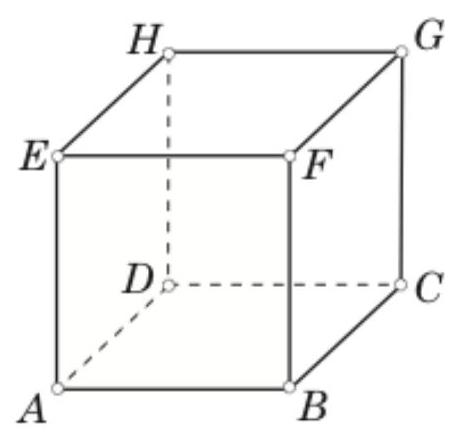
\includegraphics[max width=\textwidth, center]{2024_11_21_8b84130892fdf090117bg-1}

Uzasadnij, że trójkąty \(A M N, C N P\) i \(H P M\) są trójkątami przystającyni.\\
5. Powiemy, że liczba całkowita \(n\) jest liczbą stoneczna, jeżeli \(n=a^{2}+5 b^{2}\), gdzie liczby \(a\) i \(b\) są liczbami całkowitymi różnymi od zera. Wykaż, że jeżeli liczba \(n\) jest liczbą sloneczna, to liczba \(n^{4}\) też jest liczbą stoneczna.

\section*{Wskazówka}
Wykaż, że kwadrat liczby slonecznej jest liczbą stoneczna.\\
6. Dana jest taka liczba rzeczywista, której rozwinięcie dziesiętne jest nieskończone i składa się wyłącznie z cyfr 1, 2 i 3 . Wykaż, że jeżeli w tym rozwinięciu jest co najwyżej 2010 jedynek i co najwyżej 2010 dwójek, to dana liczba jest wymierna.

\section*{Wskazówka}
Przedstaw daną liczbę w postaci sumy dwóch liczb. Pierwsza z tych liczb ma rozwinięcie dziesiętne, w którym są wszystkie jedynki i wszystkie dwójki oraz pewna liczba trójek, a w rozwinięciu drugiej występują już tylko same trójki.\\
7. Na okręgu napisano \(n\) liczb rzeczywistych w taki sposób, że każda z tych liczb jest równa wartości bezwzględnej różnicy dwóch liczb stojących bezpośrednio za nią (patrząc zgodnie z ruchem wskazówek zegara).\\
a) Znajdź te liczby, jeśli \(n=2010\) a ich suma jest równa 1340 .\\
b) Znajdź sumę tych liczb, jeśli \(n=1000\).

\section*{Wskazówka}
Wykaż, że wszystkie napisane liczby są nieujemne. Jeśli \(x\) jest największą z nich, to jakie liczby mogą sąsiadować z \(x\) ?


\end{document}